\title{ALPSアプリケーション実行チュートリアル}

\begin{document}

\lstset{language={C++},showspaces=false,rulecolor=\color[cmyk]{0, 0.29,0.84,0}}

\begin{frame}
  \titlepage
\end{frame}

\section*{Outline}
\begin{frame}
   \tableofcontents
\end{frame}

\section{XML入門}
\subsection*{{\protect\color{red}●}{\protect\color{blue}●}}

\begin{frame}{ALPSによるシミュレーション --- ワークフロー}
  \begin{center}
    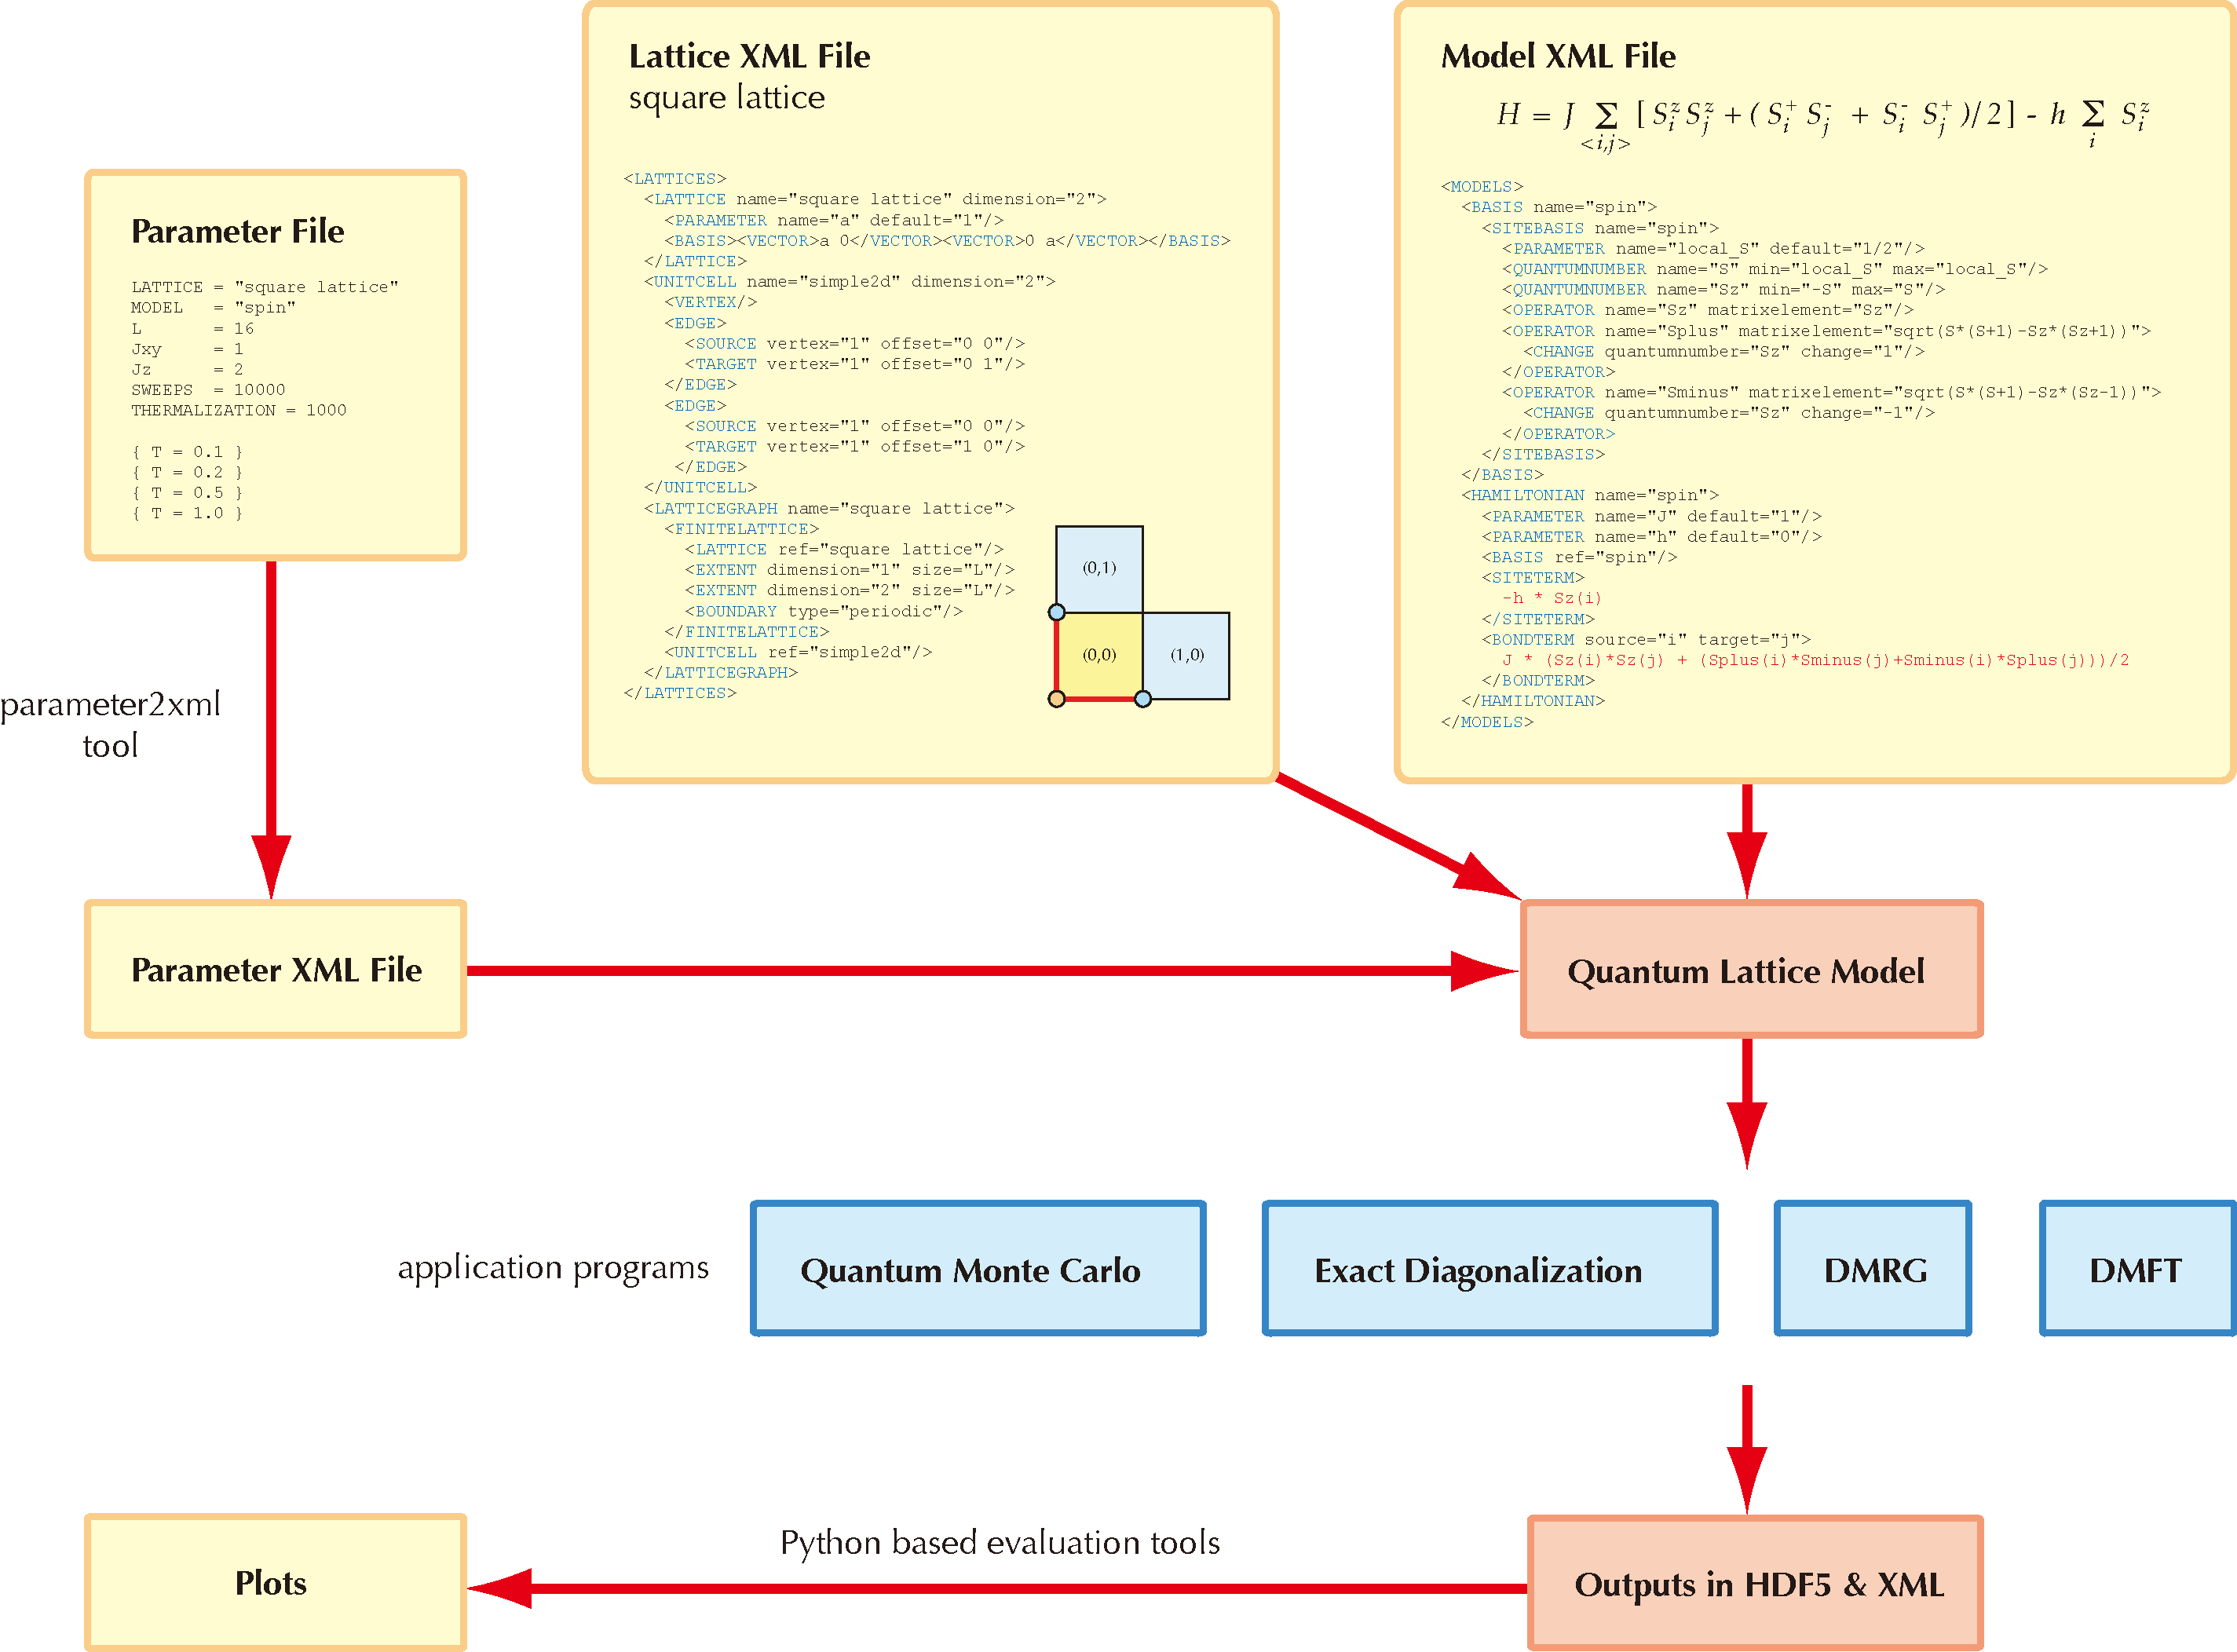
\includegraphics[height=0.8\textheight]{workflow.pdf}
  \end{center}
\end{frame}

\begin{frame}{XMLの基礎}
  \begin{itemize}
  \item XML = e{\color{red} X}tensible {\color{red} M}arckup {\color{red} L}anduage
  \item 構造化文書を作成するのに適している
  \item 「タグ」を使って、文章の構造を記述
  \item 大文字と小文字は区別される
  \item XMLの例: HTML (XHTML)
  \begin{center}
    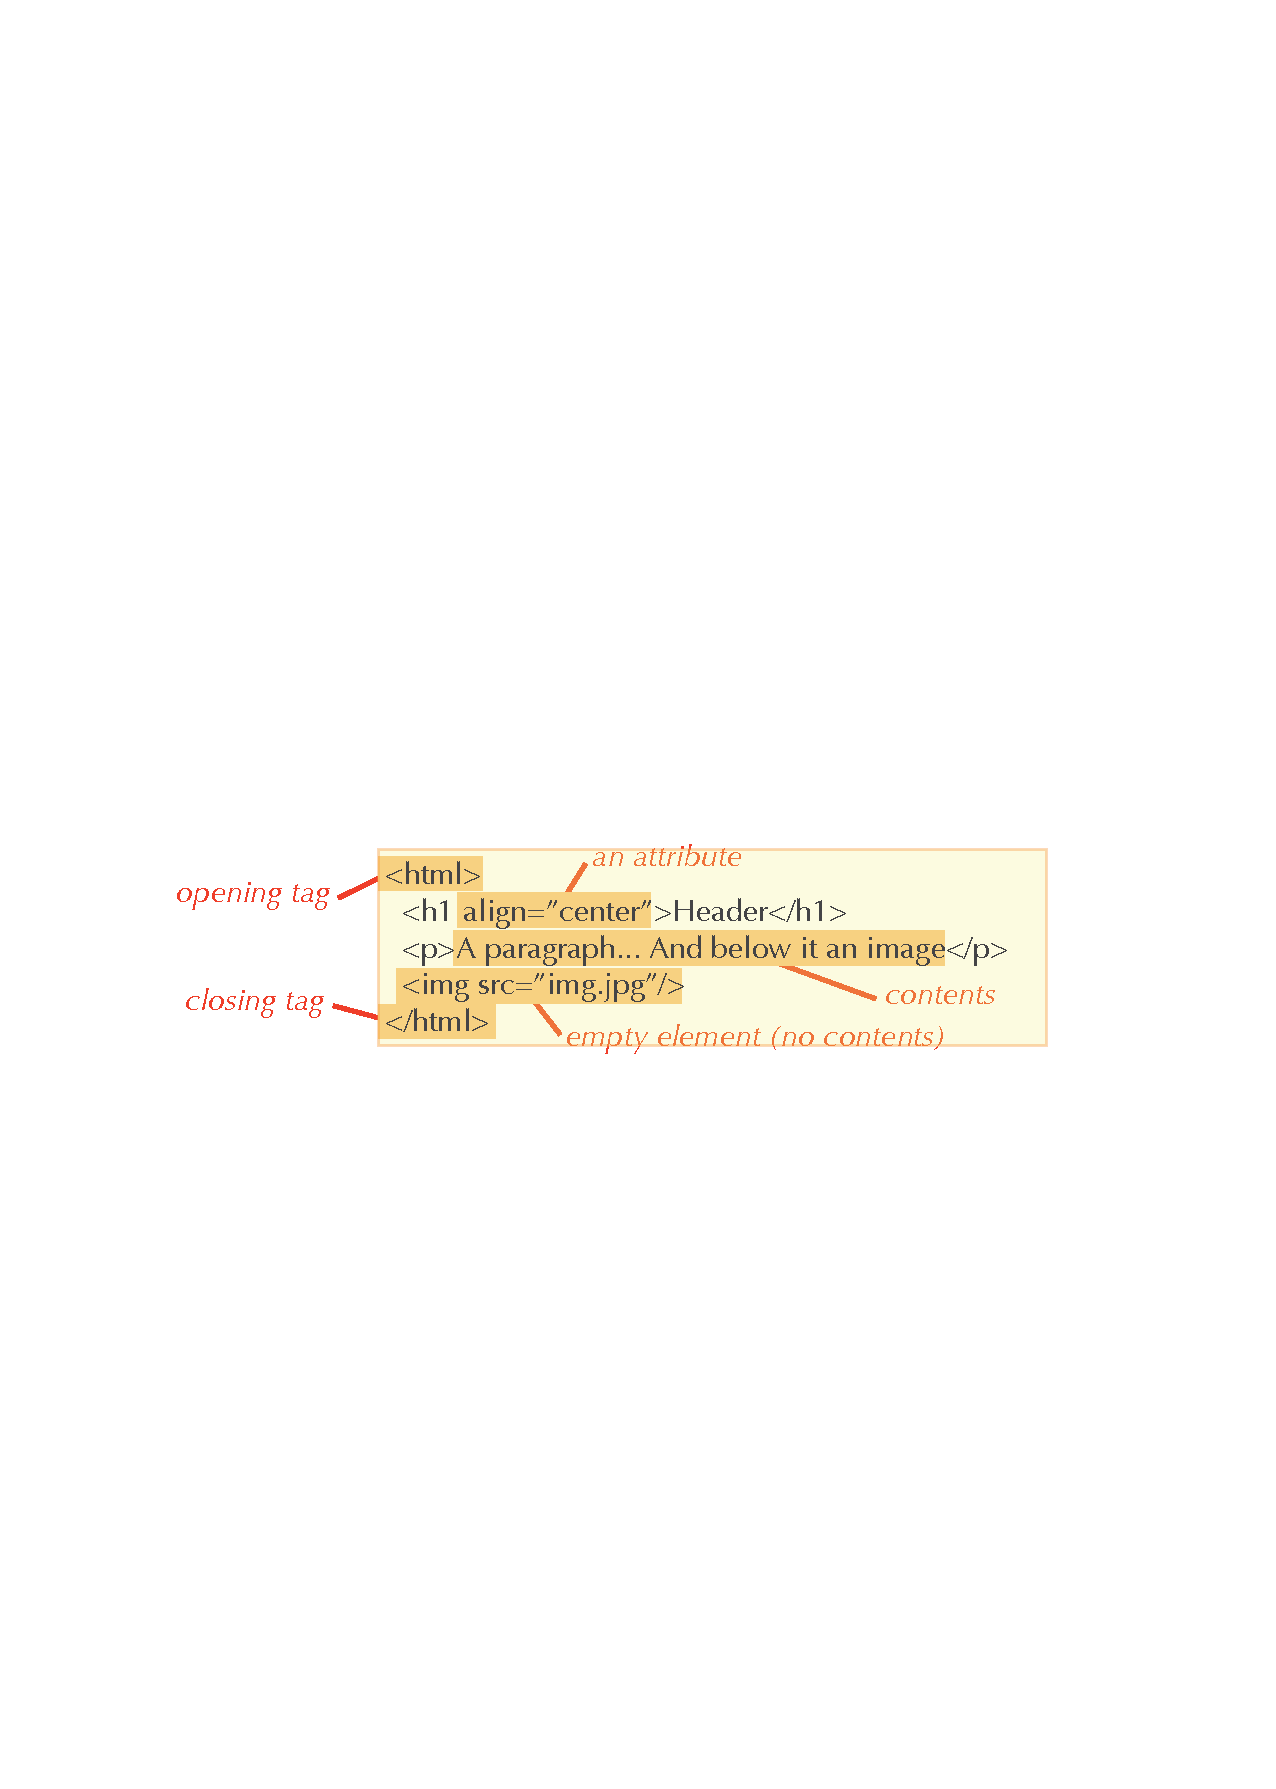
\includegraphics[height=0.3\textheight]{xml1.pdf}
  \end{center}
  \end{itemize}
\end{frame}

\begin{frame}{XMLの文法}
  \begin{itemize}
  \item 「開始タグ」には対応する「終了タグ」が必要
  \item ある要素の「開始タグ」と終了タグは共通の親ノードに含まれなければならない
  \item XMLの「木」表示
  \begin{center}
    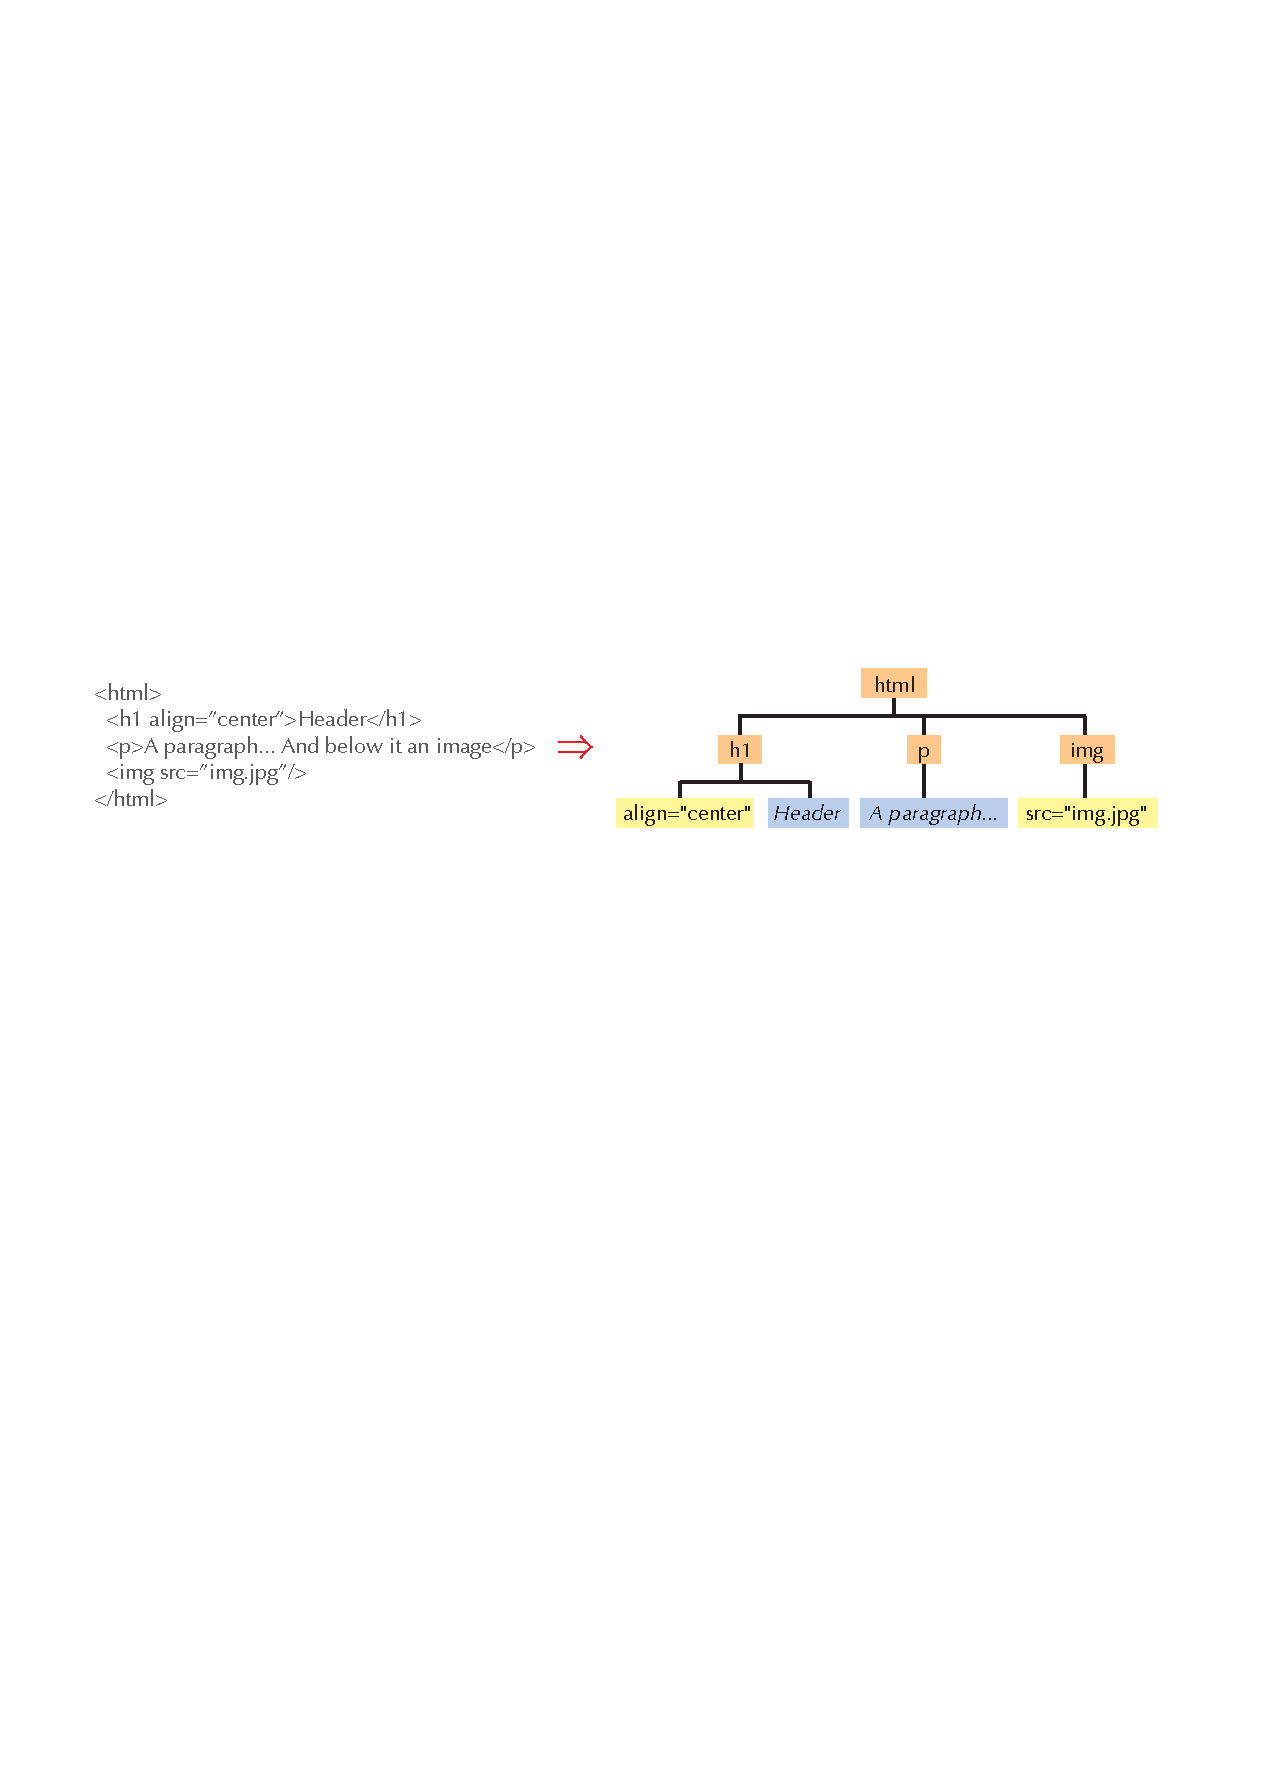
\includegraphics[width=\textwidth]{xml2.pdf}
  \end{center}
  \item XMLでは、ユーザが独自のタグ(要素の名前)を定義することが可能 \\
    (参考: Document Type Definition (DTD), XML Schema)
  \end{itemize}
\end{frame}

\begin{frame}{なぜXMLを使うのか?}
  \begin{center}
    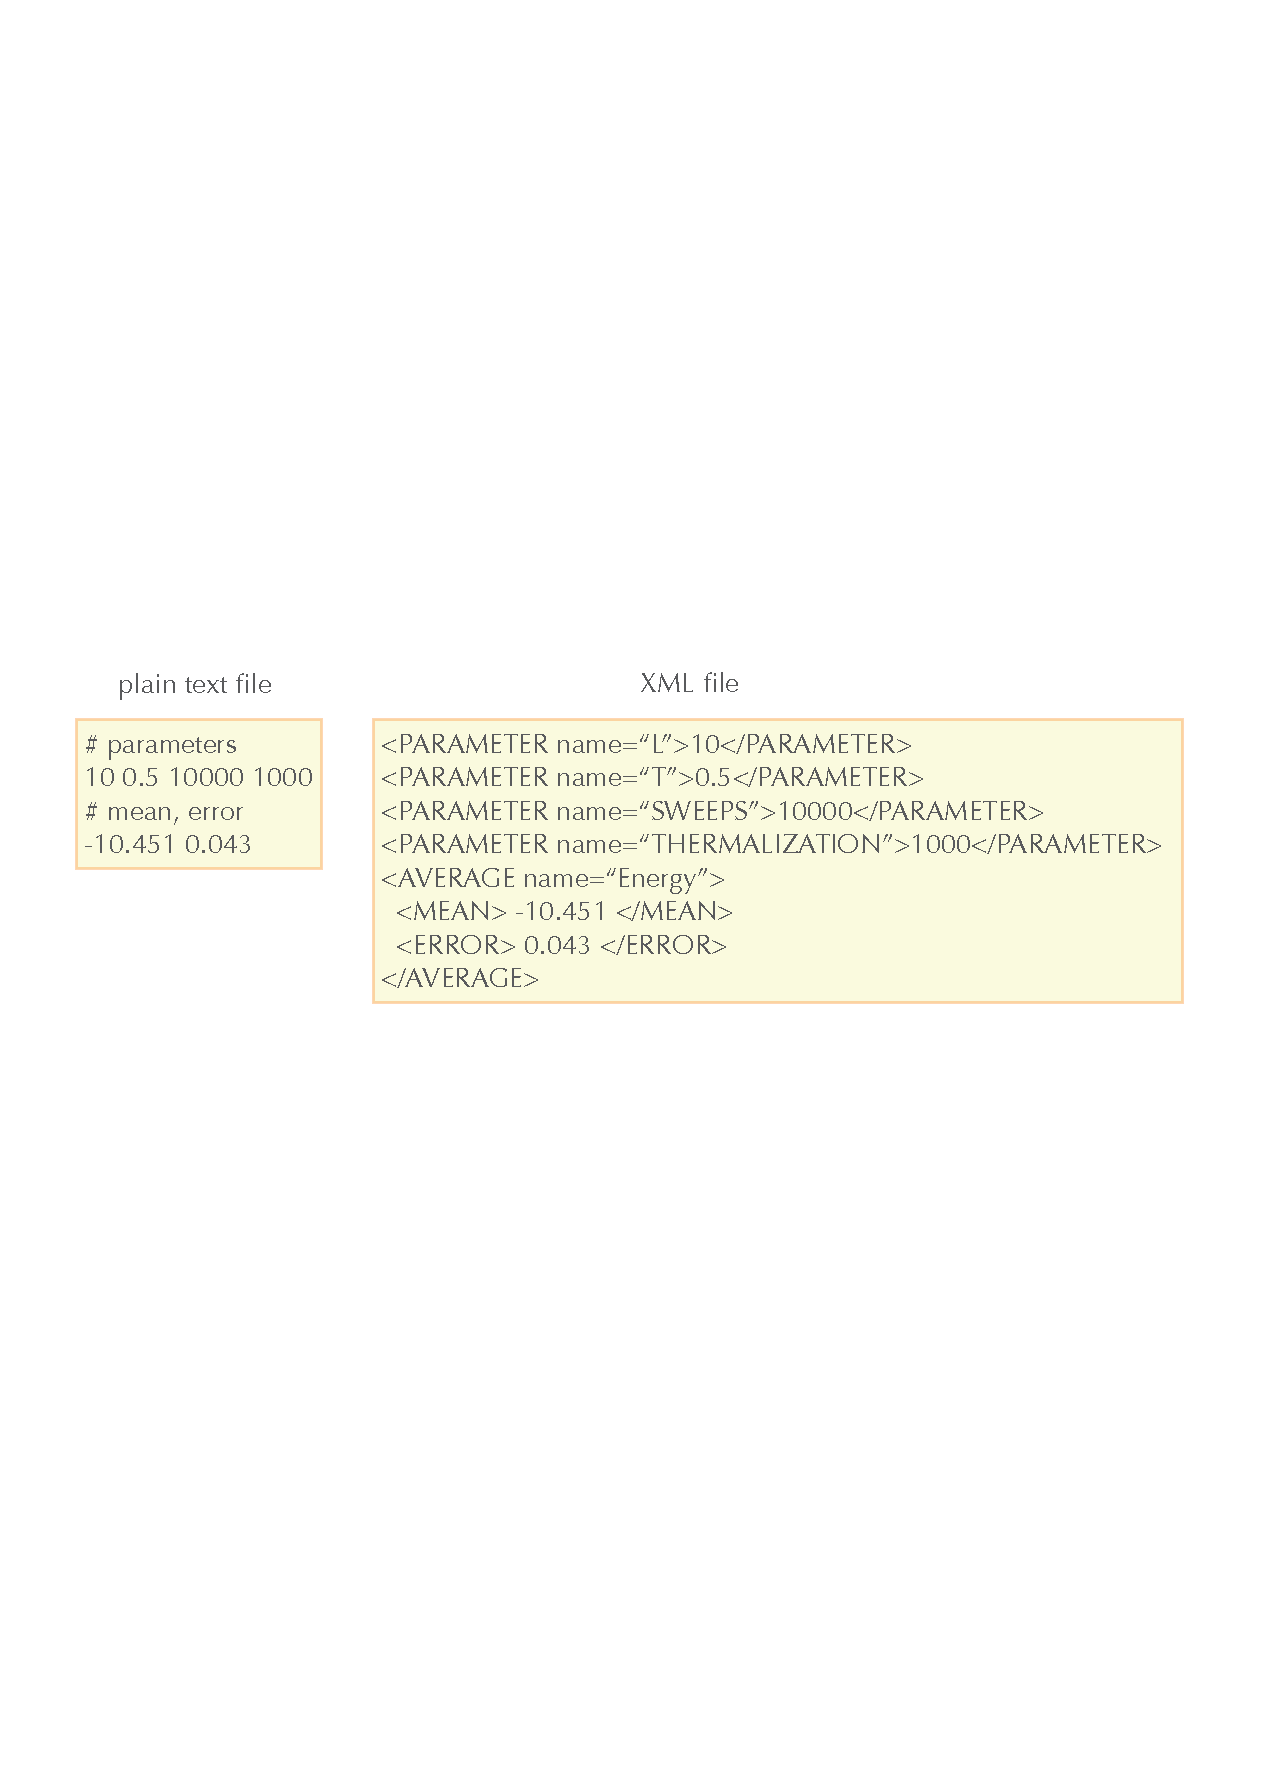
\includegraphics[width=.8\textwidth]{xml3.pdf}
  \end{center}
  \begin{itemize}
  \item 人間にはどちらが読みやすい?
  \item 機械にはどちらがよみやすい?
  \item 数年後に読んで理解できるのはどっち?
  \end{itemize}
\end{frame}

\begin{frame}{データ形式の拡張性}
  \begin{itemize}
  \item 新しいパラメータを追加すると、、、
  \begin{center}
    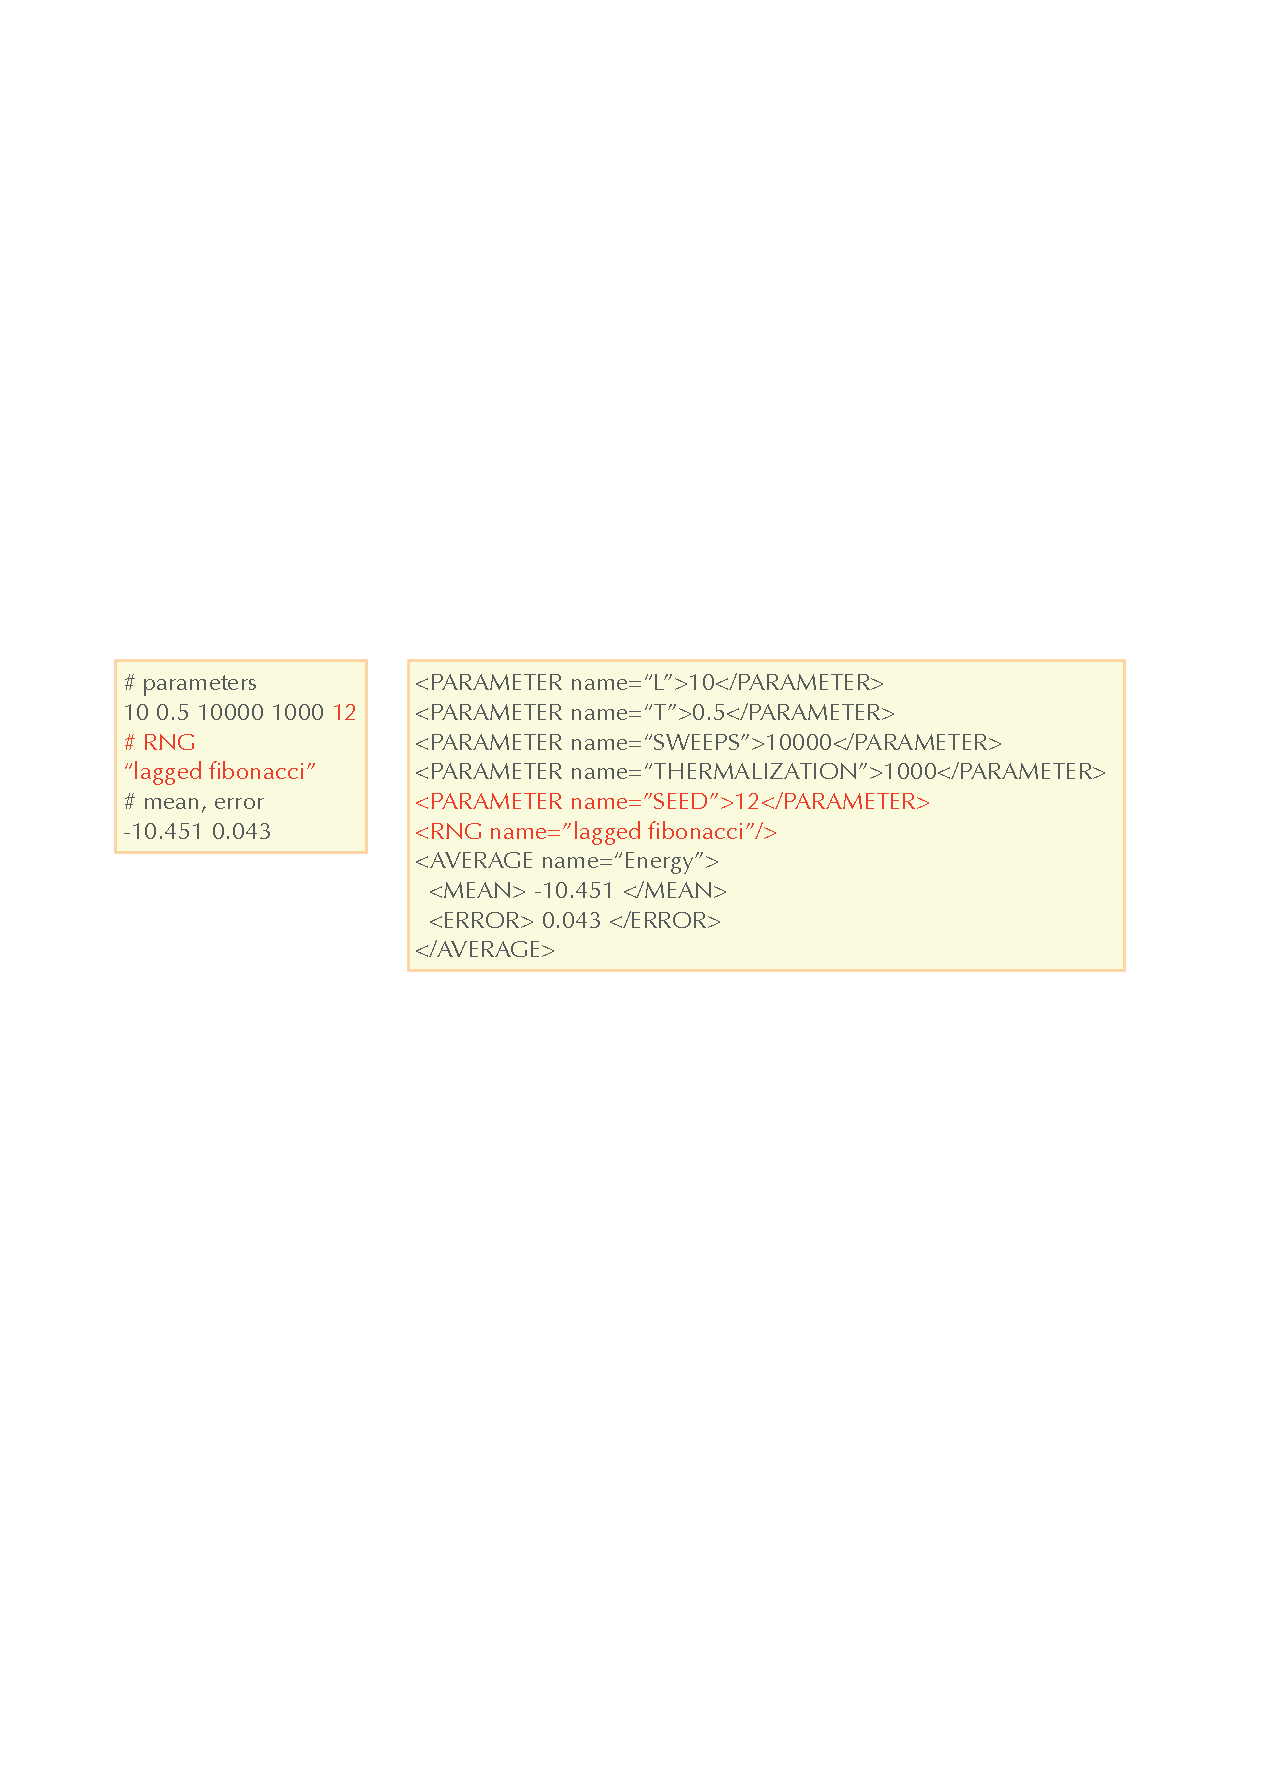
\includegraphics[width=.8\textwidth]{xml4.pdf}
  \end{center}
  \item テキスト形式の場合、これまでのプログラムは動かなくなる
  \item XMLの場合には問題ない (必要のないパラメータは読まれない)
  \end{itemize}
\end{frame}

\section{ALPSシミュレーションの流れ}
\subsection*{{\protect\color{red}●}{\protect\color{blue}●}}

\begin{frame}{シミュレーションの入出力}
  \begin{itemize}
  \item 典型的には、一つのシミュレーションは複数のパラメータセットからなる \\ (異なる温度など)
    \begin{itemize}
    \item 「ジョブ(job)」: シミュレーション全体、「タスク」の集合
    \item 「タスク(task)」(または「simulation」):– 一つのパラメータセットに対する計算、「ラン」の集合
    \item 「ラン(run)」(または「clone」): 異なる乱数の種に対する個々の計算
    \end{itemize}
  \item XML入力ファイルと出力ファイル
  \begin{center}
    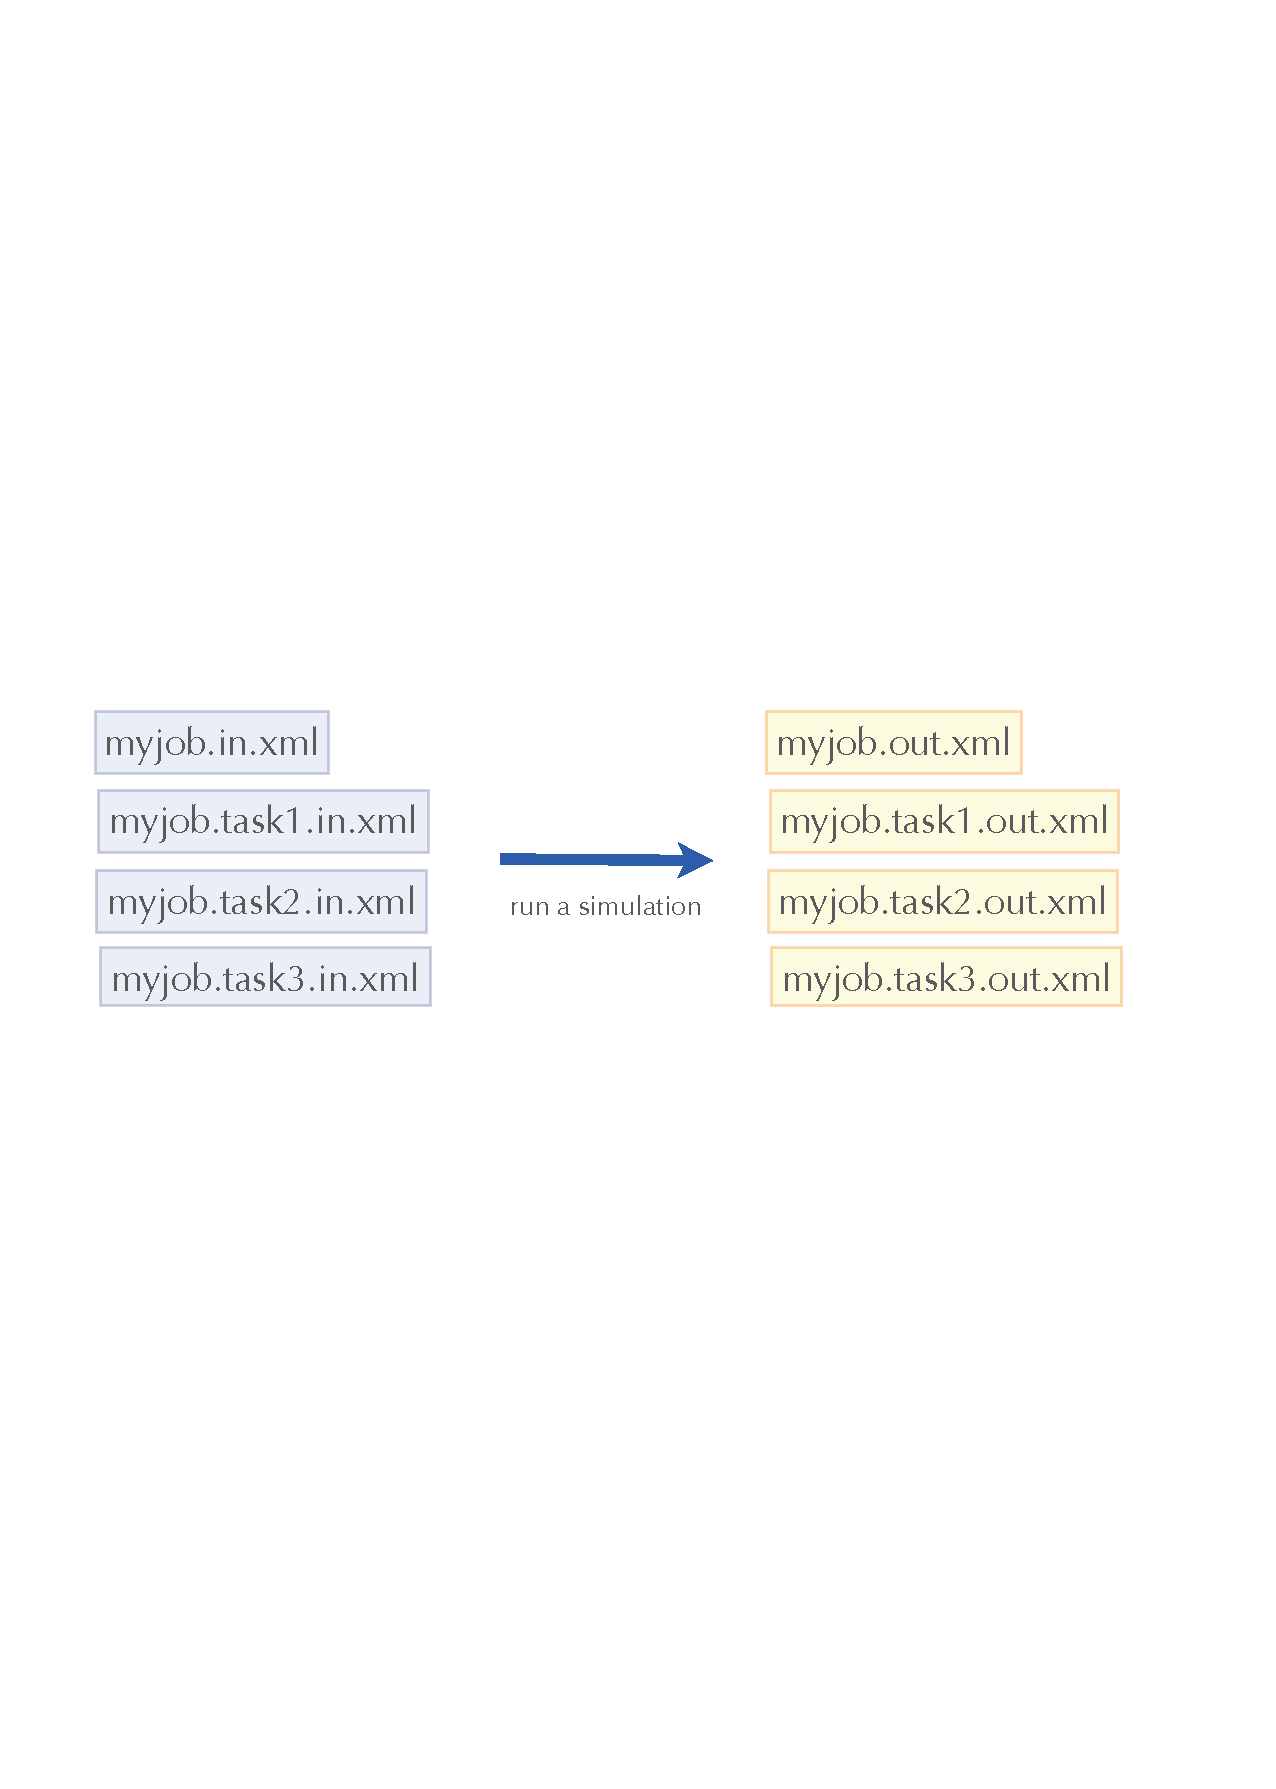
\includegraphics[width=.55\textwidth]{simulation1.pdf}
  \end{center}
  \end{itemize}
\end{frame}

\begin{frame}{Job XML ファイル}
  \begin{center}
    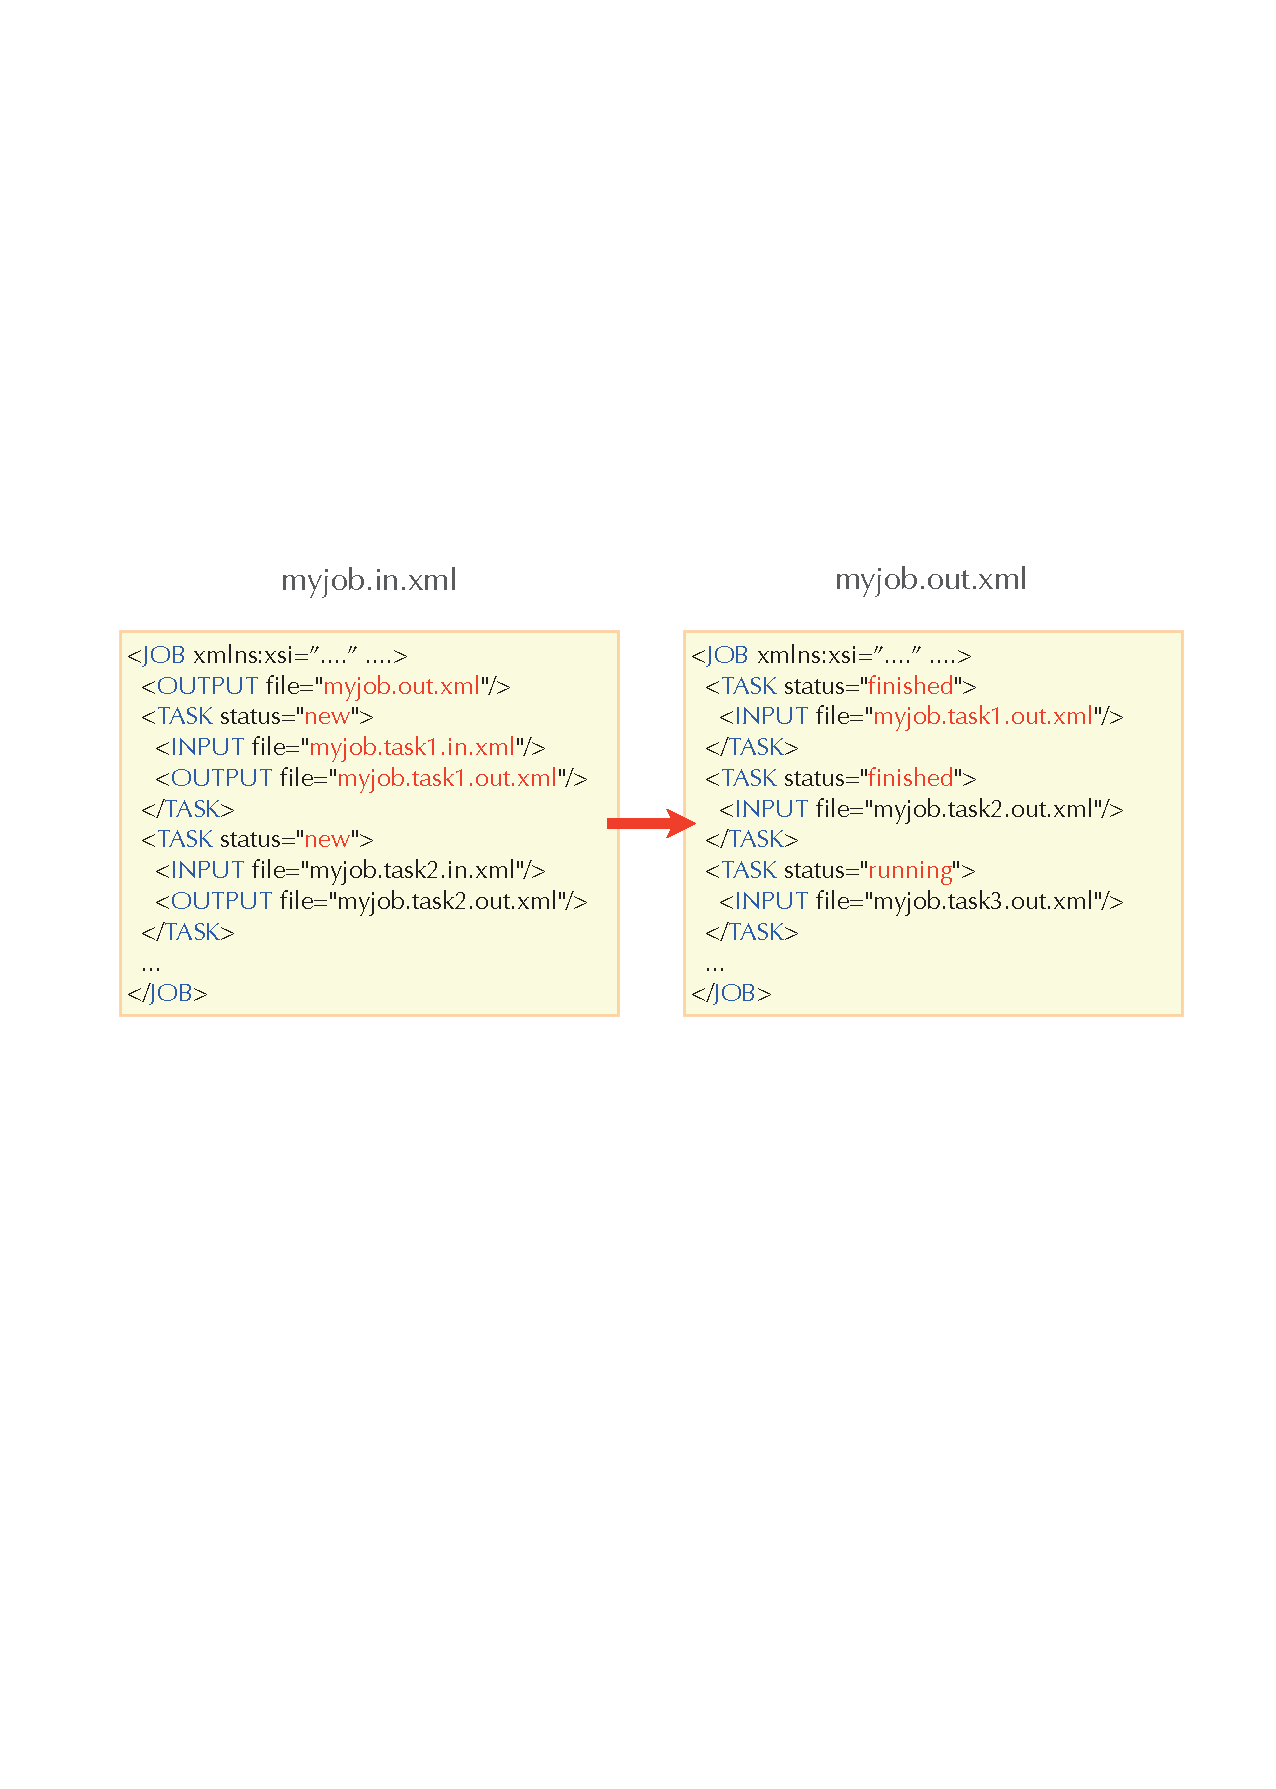
\includegraphics[height=.6\textheight]{simulation2.pdf}
  \end{center}
\end{frame}

\begin{frame}{Task XML ファイル}
  \begin{center}
    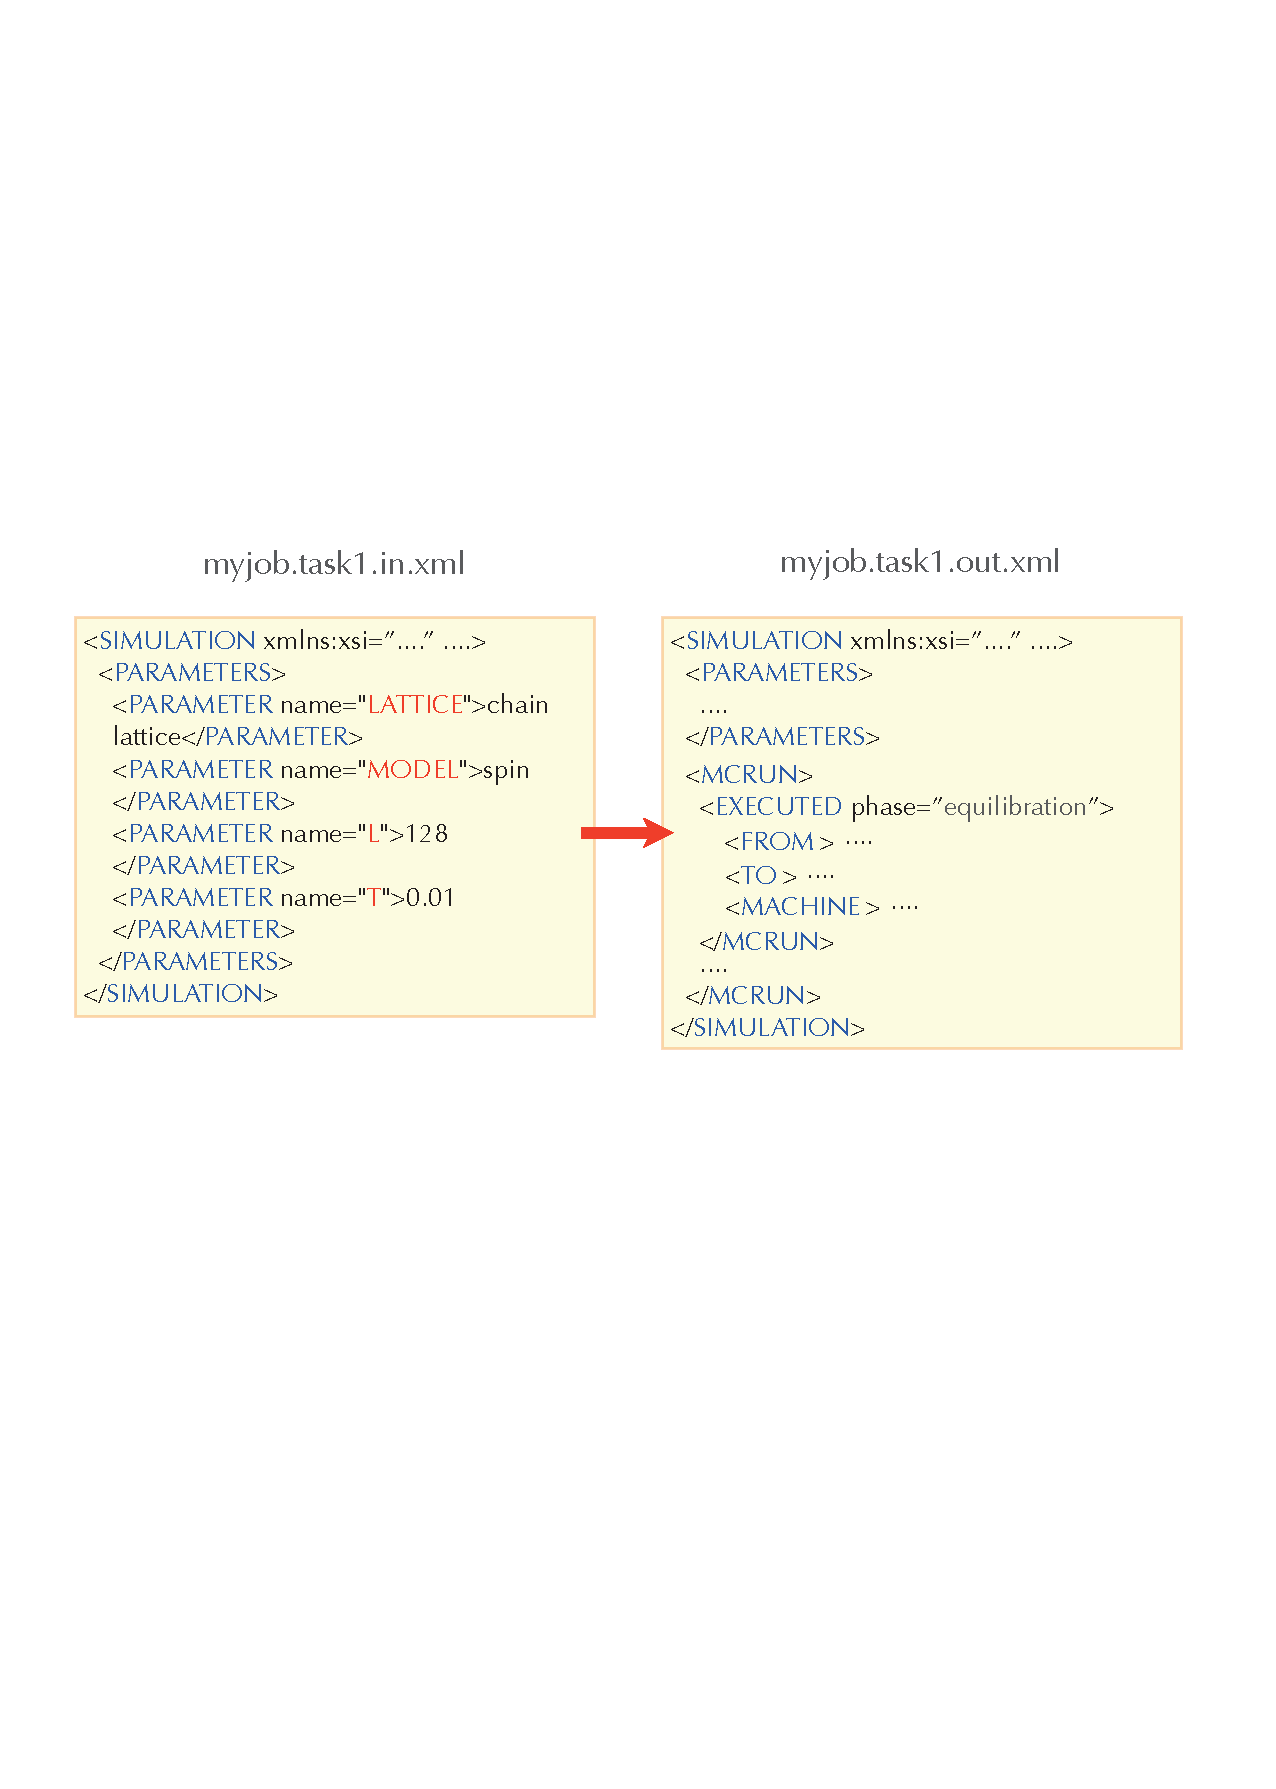
\includegraphics[height=.6\textheight]{simulation3.pdf}
  \end{center}
\end{frame}

\begin{frame}{parameter2xml ツール}
  \begin{itemize}
  \item パラメータセットを簡易形式で書いて、parameter2xmlツールでXMLに変換する
  \begin{center}
    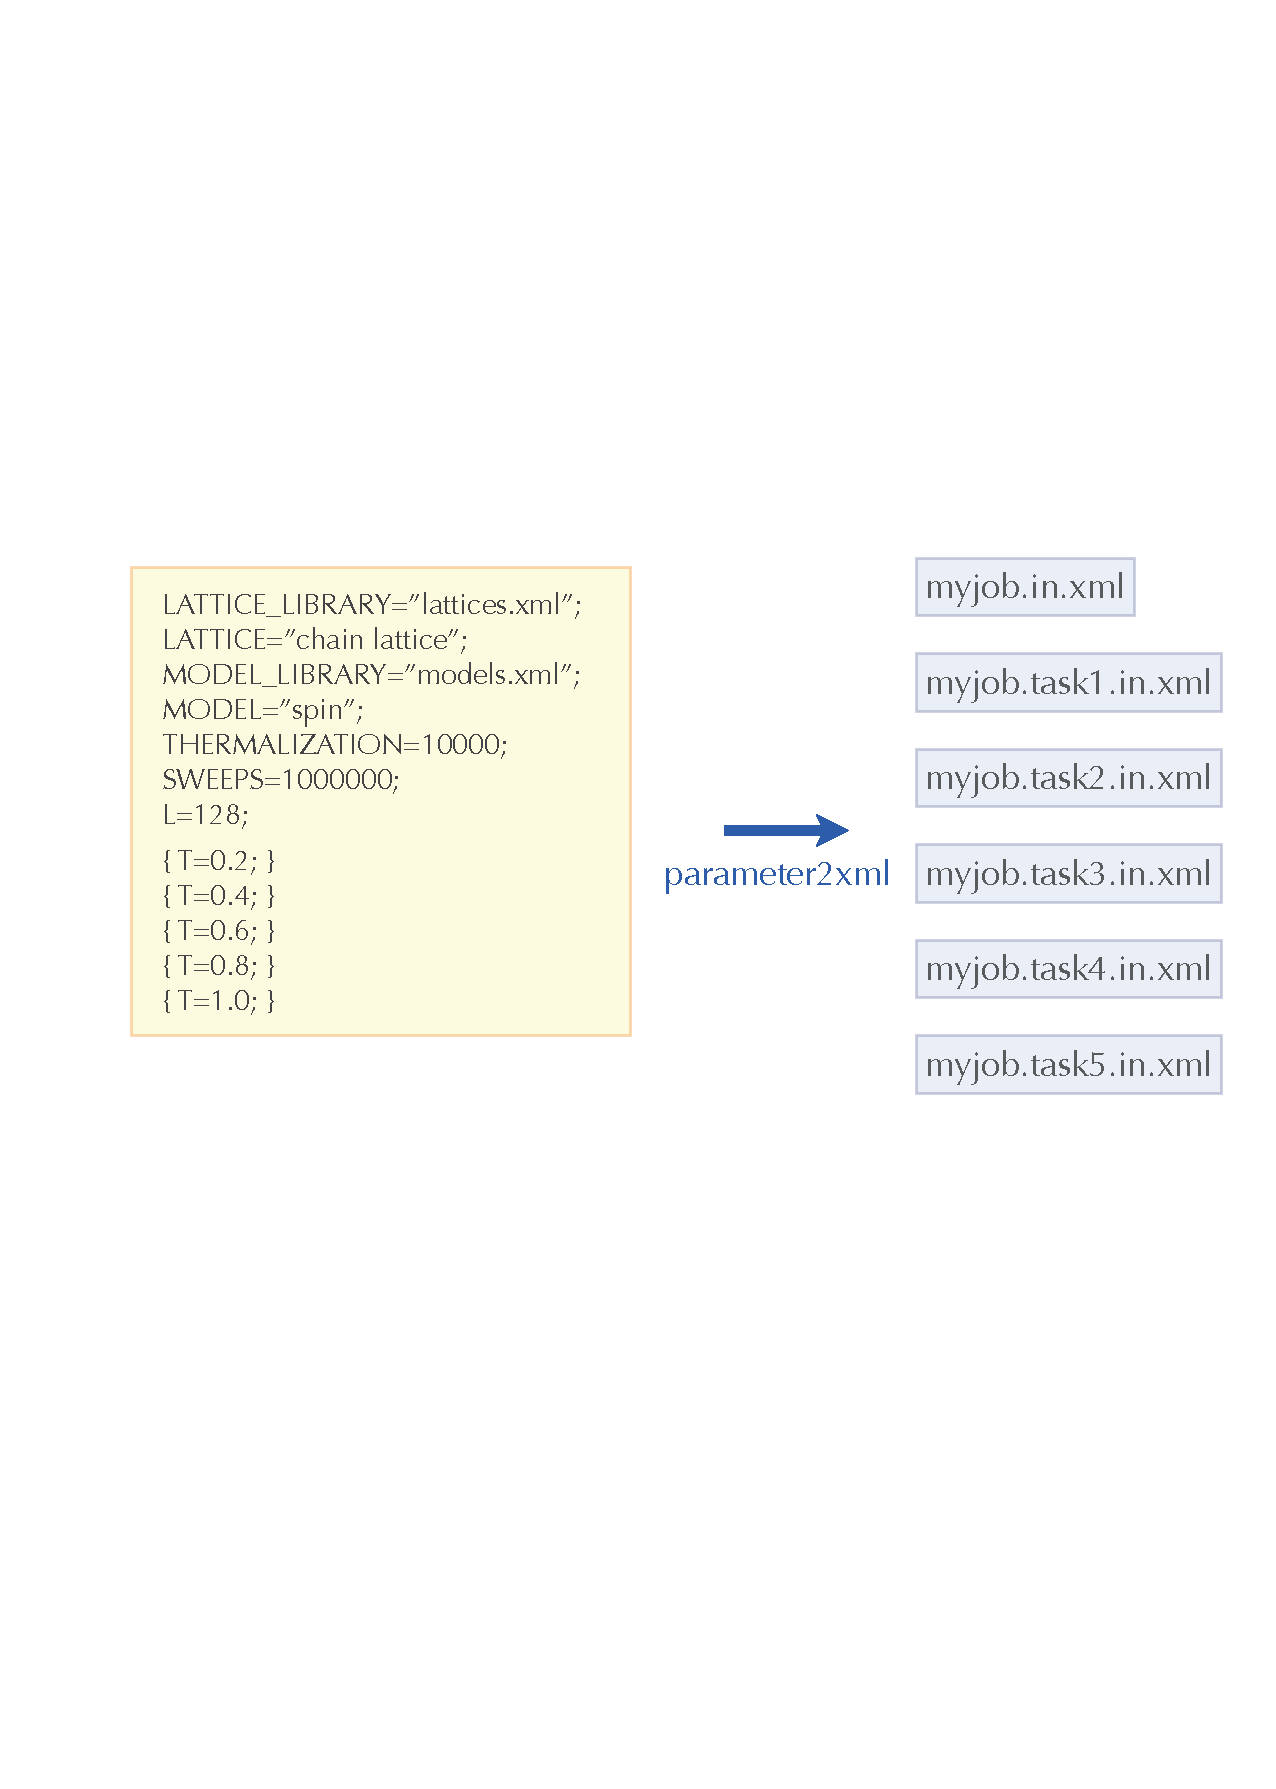
\includegraphics[height=.6\textheight]{simulation4.pdf}
  \end{center}
  \item pyalps (後述)では、pyalps.writeInputFiles() メソッドが利用できる
  \end{itemize}
\end{frame}

\begin{frame}{格子とモデルの指定}
  \begin{itemize}
  \item 格子とモデルを指定するための特別なパラメータ
  \begin{center}
    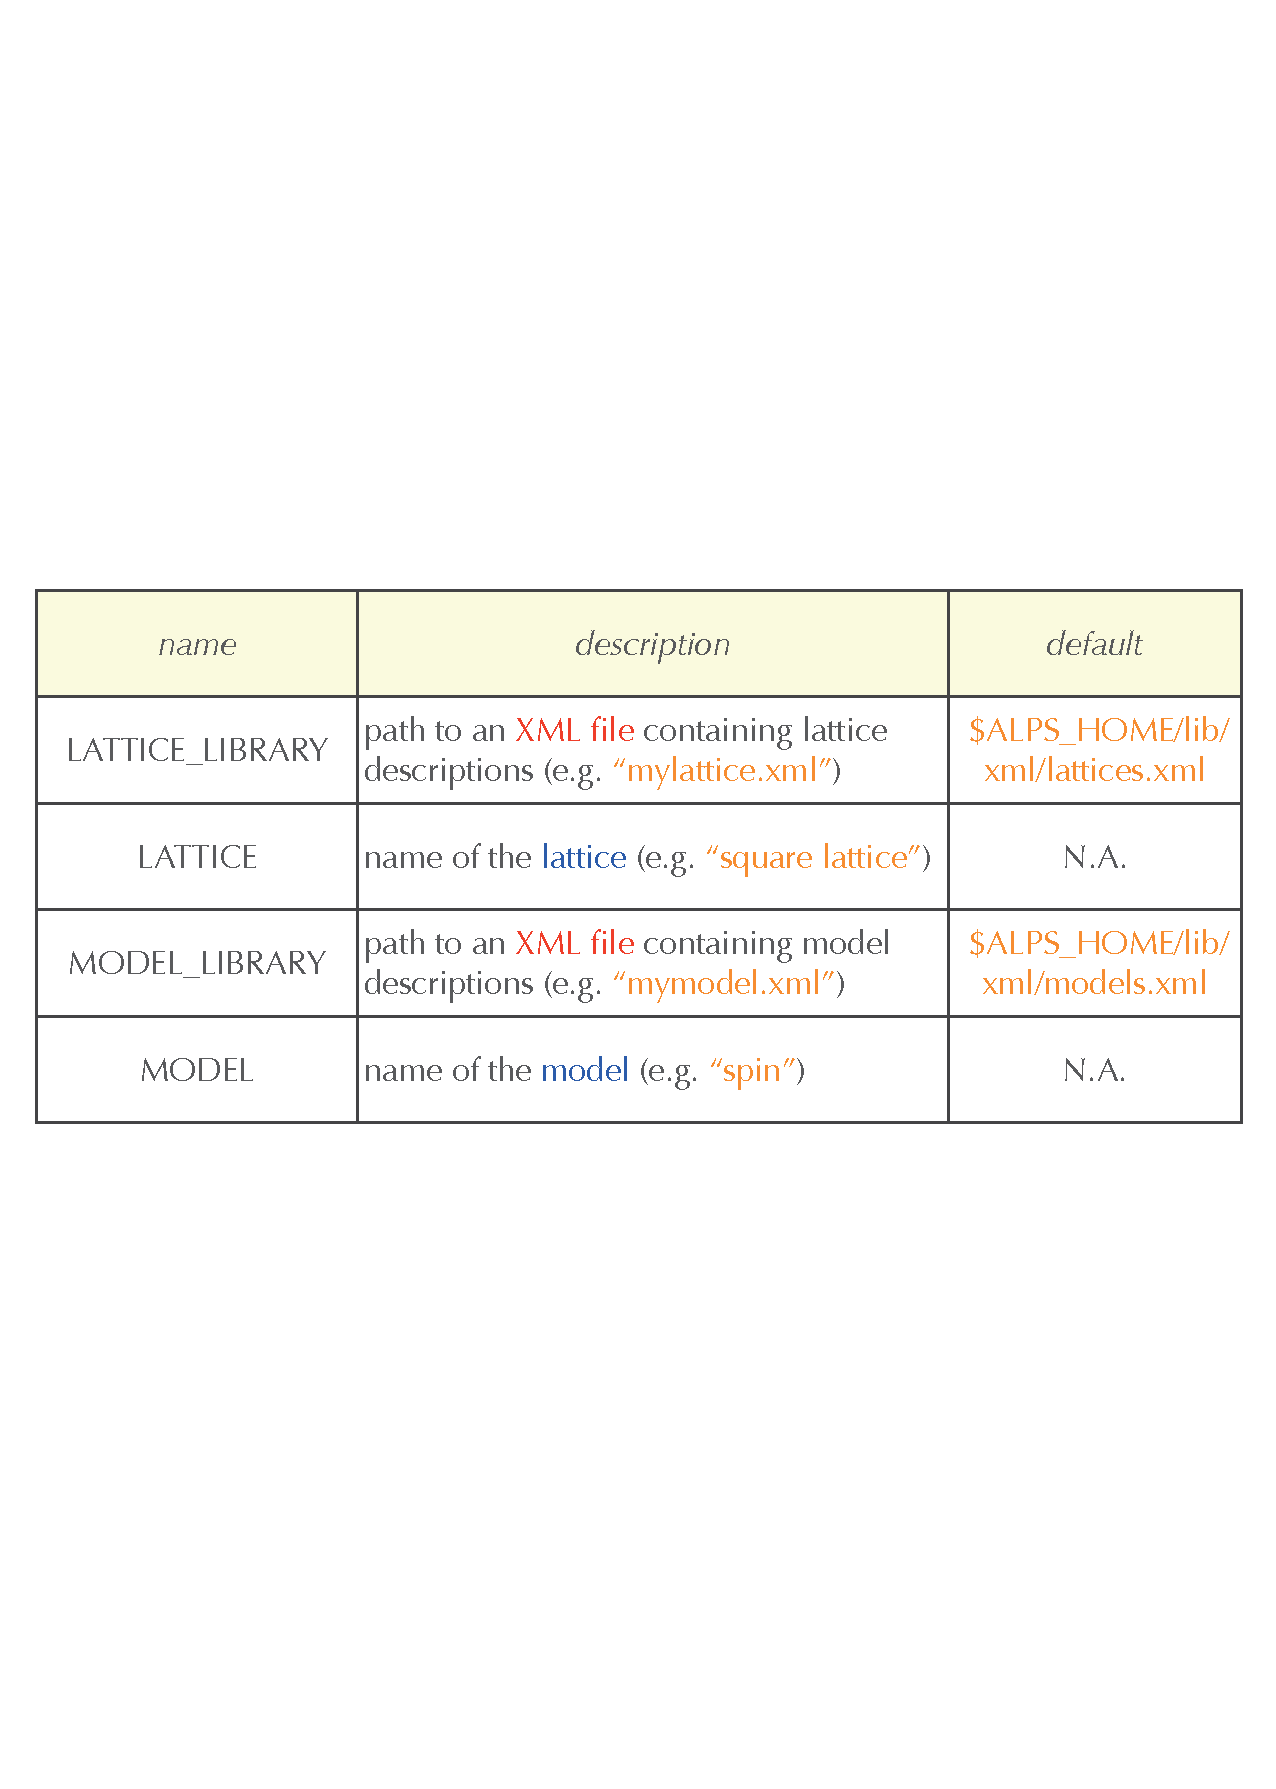
\includegraphics[height=4cm]{simulation5.pdf}
  \end{center}
  \end{itemize}
\end{frame}

\begin{frame}[t,fragile]
  \frametitle{パラメータファイルでの数式の使用}
  \begin{columns}[T]
    \begin{column}{.5\textwidth}
      \begin{itemize}
        %\begin{itemize}
        \item 改行, セミコロン, コンマで変数を区別
        \item 四則演算、初等関数(sin, cos, expなど)が使える
        \item $\pi$ (PI), 虚数単位(I)などを文字で指定
        \item C 風, C++風のコメント
        \item \{ \} で囲んだ変数は異なるセット
        \item 「循環参照」がある場合にはエラーになる
        %\end{itemize}
      \end{itemize}
    \end{column}
    \begin{column}{.5\textwidth}
    \begin{lstlisting}
LATTICE = "chain lattice";
L = 16,
SEED = 2873
// C++ style comment
SWEEPS = 4096;
THERMALIZATION = SWEEPS/8;
/* C style comment */
{ T = 2; Sq = 2*PI/3; }
{ T = 1.8; }
    \end{lstlisting}
    \end{column}
  \end{columns}
\end{frame}

\section{ALPSチュートリアル}

\begin{frame}
  \frametitle{ディレクトリ構成 (例)}
  \begin{tabular}{ll}
    /opt/nano/alps/alpsvars.sh & \\
    \hspace*{3em} ALPS環境変数(\$PATH, \$ALPS\_HOME等)設定スクリプト \\
    /opt/nano/alps/tutorials & \\
    \hspace*{3em} アプリケーションのチュートリアル用入出力ファイル \\
    /opt/nano/alps/notebook & \\
    \hspace*{3em} iPythonノートブックによるチュートリアル
  \end{tabular}
  \begin{alertblock}{}
    alpsvars.shはALPSがインストールされたスパコン全てに用意されています \\
    {\footnotesize \url{https://github.com/wistaria/installer/wiki}}
\end{alertblock}
\end{frame}

\begin{frame}[fragile]
  \frametitle{実習準備}
  \begin{enumerate}
  \item 実習システムにログイン
\begin{semiverbatim}
\$ ssh -X guest{\color{red}XX}@{\color{red}hostname}
\end{semiverbatim}
  \item 環境変数の設定
\begin{semiverbatim}
\$ source /opt/nano/alps/alpsvars.sh
\end{semiverbatim}
  \item チュートリアルをコピー
\begin{semiverbatim}
\$ cp -rp /opt/nano/alps/tutorials/ .
\end{semiverbatim}
  \item iPythonノートブックをコピー
\begin{semiverbatim}
\$ cp -rp /opt/nano/alps/notebook/ .
\end{semiverbatim}
  \end{enumerate}
\end{frame}

\begin{frame}[fragile]
  \frametitle{ALPSの実行シナリオ}
  \begin{enumerate}
  \item コマンドライン(旧来からの方法)
\begin{semiverbatim}
\$ parameter2xml \textit{param}
\$ loop \textit{param}.in.xml
\end{semiverbatim}
  \item シェルスクリプト(バッチ処理)
  \item {\color{red}Python} (インタラクティブ or バッチ)
    \begin{itemize}
    \item パラメータの準備からグラフ作成まで統一的に
    \item 対話的にもバッチコマンドとしても実行可能
    \item グラフの作成も、PythonのMatplotlibを用いる
    \end{itemize}
  \item {\color{red}IPython notebook}
    \begin{itemize}
    \item ブラウザ上でPythonコマンドを実行
    \item 入力、出力を「ノートブック」としてまとめて保存
    \item グラフの描画もブラウザ上で可能
    \end{itemize}
  \item VisTrails (履歴管理ツール)
  \end{enumerate}
\end{frame}

\begin{frame}
  \frametitle{ALPSアプリケーション}
  \begin{description}
  \item[fulldiag] {\color{red} 厳密対角化(全対角化法)}
  \item[sparsediag] {\color{red} 厳密対角化(Lanczos法)}
  \item[spinmc] 古典モンテカルロ法
  \item[loop] {\color{red} 量子モンテカルロ法(ループアルゴリズム)}
  \item[dirloop\_sse] {\color{red} 量子モンテカルロ(向き付きループアルゴリズム)}
  \item[worm] 量子モンテカルロ(ワームアルゴリズム)
  \item[dmrg,tebd] 密度行列繰り込み群
  \item[hirshfye,interaction,hybridization] 動的平均場近似のQMCソルバ
  \end{description}
\end{frame}

\begin{frame}[fragile]
  \frametitle{コマンドライン実行 (厳密対角化 ed-01)}
  \begin{enumerate}
  \item 実習システムにログイン
\begin{semiverbatim}
\$ ssh -X guest{\color{red}XX}@{\color{red}hostname}
\end{semiverbatim}
  \item (必要に応じて)計算ノードにログイン
  \item 環境変数の設定
\begin{semiverbatim}
\$ source /opt/nano/alps/alpsvars.sh
\end{semiverbatim}
  \item 入力XMLファイルの準備
\begin{semiverbatim}
\$ cd tutorials/ed-01-sparsediag
\$ parameter2xml parm1a
\end{semiverbatim}
  \item sparsediagの実行
\begin{semiverbatim}
\$ sparsediag --write-xml parm1a.in.xml
\end{semiverbatim}
  \item 結果はparm1a.task1.out.xmlに出力される
  \end{enumerate}
\end{frame}

\begin{frame}[fragile]
  \frametitle{シェルスクリプトによる実行 (厳密対角化 ed-01)}
  \begin{enumerate}
  \item 実習システムにログイン
\begin{semiverbatim}
\$ ssh -X guest{\color{red}XX}@{\color{red}hostname}
\end{semiverbatim}
  \item (必要に応じて)計算ノードにログイン
  \item シェルスクリプト(バッチファイル)の準備
\begin{semiverbatim}
\$ cd tutorials/ed-01-sparsediag
\$ vi batch.sh
\end{semiverbatim}
  \item batch.sh の中身
\begin{lstlisting}
#!/bin/sh
source /opt/nano/alps/alpsvars.sh
parameter2xml parm1a
sparsediag --write-xml parm1a.in.xml
\end{lstlisting}
  \item シェルスクリプトを実行 (あるいはバッチキューに投入)
\begin{semiverbatim}
\$ sh batch.sh
\end{semiverbatim}
  \end{enumerate}
\end{frame}

\begin{frame}[fragile]
  \frametitle{Pythonでの対話的実行 (厳密対角化 ed-01)}
  \begin{enumerate}
  \item 実習システムにログイン
\begin{semiverbatim}
\$ ssh -X guest{\color{red}XX}@{\color{red}hostname}
\end{semiverbatim}
  \item (必要に応じて)計算ノードにログイン
  \item 環境変数の設定
\begin{semiverbatim}
\$ source /opt/nano/alps/alpsvars.sh
\end{semiverbatim}
  \item IPythonの起動
\begin{semiverbatim}
\$ cd tutorials/ed-01-sparsediag
\$ ipython
\end{semiverbatim}
  \item \href{http://alps.comp-phys.org/mediawiki/index.php/ALPS_2_Tutorials:ED-01_SparseDiagonalization/ja#Python.E3.81.A7.E3.81.AE.E5.AE.9F.E8.A1.8C}{チュートリアルページ}にしたがって、コマンドを実行 (コマンドはTABで補完できる)
  \end{enumerate}
\end{frame}

\begin{frame}[fragile]
  \frametitle{Pythonでのバッチ実行 (厳密対角化 ed-01)}
  \begin{enumerate}
  \item 実習システムにログイン
\begin{semiverbatim}
\$ ssh -X guest{\color{red}XX}@{\color{red}hostname}
\end{semiverbatim}
  \item (必要に応じて)計算ノードにログイン
  \item 環境変数の設定
\begin{semiverbatim}
\$ source /opt/nano/alps/alpsvars.sh
\end{semiverbatim}
  \item バッチ実行
\begin{semiverbatim}
\$ cd tutorials/ed-01-sparsediag
\$ python tutorial1a.py
\end{semiverbatim}
  \end{enumerate}
\end{frame}

\begin{frame}[fragile,shrink=10]
  \frametitle{IPython notebookでの実行 (厳密対角化 ed-01)}
  \begin{enumerate}
  \item 実習システムにログイン
\begin{semiverbatim}
\$ ssh -X guest{\color{red}XX}@{\color{red}hostname}
\end{semiverbatim}
  \item IPython notebookサーバの起動
\begin{semiverbatim}
\$ source /opt/nano/alps/alpsvars.sh
\$ cd notebook/jp
\$ ipython notebook --no-browser --pylab inline
\end{semiverbatim}
  \item 起動時に出力されるポート番号(8888等)を控えておく
  \item 手元のPCでもう一つポートフォワーディング付きでSSHセッションを開く
\begin{semiverbatim}
\$ ssh guest{\color{red}XX}@{\color{red}hostname} -L 8888:{\color{red}hostname}:8888
\end{semiverbatim}
  \item PCでブラウザを起動し、http://localhost:8888 を開く
  \item ED-01\_SparseDiagonalization.ipynb を開き、[Shift+Return] で実行していく
  \end{enumerate}
  注: フロントエンドでの実行のため、他の人のジョブと干渉して遅くなる場合がある
\end{frame}

\begin{frame}{実行結果の確認}
  \begin{itemize}
    \item 実行結果(JOB XMLファイル、TASK XMLファイル)は、webブラウザで直接開いて中身を見ることも可能
      \begin{itemize}
      \item 例(Linux): firefox parm1a.task1.out.xml
      \item 例(Mac OS X): open -a safari parm1a.task1.out.xml
      \end{itemize}
  \end{itemize}
\end{frame}

\begin{frame}{シミュレーションの並列実行}
  \begin{itemize}
    \item パラメータセットに関する並列実行が可能 (embarassingly parallel)
    \item アプリケーションによって、ALPS parallelizing スケジューラか、ALPS/parapack スケジューラのいずれかが使われている (オプション -l により確認可)
    \item ALPS parallelizaing スケジューラ (spinmc等)
      \begin{itemize}
        \item OpenMPスレッド並列には対応していない。MPI並列のみ
        \item MPI実行例(4プロセス): \\ {\tt {\color{red} mpirun -np 4} spinmc {\color{red} --mpi} parm2a.in.xml}
      \end{itemize}
    \item ALPS/parapack スケジューラ (loop等)
      \begin{itemize}
        \item OpenMPスレッド並列とMPI並列に対応。デフォルトで自動的にスレッド並列実行
        \item 実行例(16スレッド): \\ {\tt loop {\color{red} -r 16} parm2c.in.xml}
      \end{itemize}
  \end{itemize}
\end{frame}

\begin{frame}{厳密対角化チュートリアル}
  \begin{itemize}
  \item \href{http://alps.comp-phys.org/mediawiki/index.php/ALPS_2_Tutorials:ED-01_SparseDiagonalization/ja}{ED-01 Sparse Diagonalization (Lanczos)
}

    $S=1$の量子1次元系(サイト数4)について, Lanczos法により固有値を求め, 固有値, 相関関数などを出力する.

  \item \href{http://alps.comp-phys.org/mediawiki/index.php/ALPS_2_Tutorials:ED-02_Gaps/ja}{ED-02 Spin gaps of 1D quantum systems}
    
    $S=1$の量子1次元系(サイト数4--14)について, Lanczos法で固有値計算を行う. 求めたエネルギー固有値からエネルギーギャップを求めプロットする.

  \item \href{http://alps.comp-phys.org/mediawiki/index.php/ALPS_2_Tutorials:ED-03_Spectra/ja}{ED-03 Spectra of 1D quantum systems}

    次の2種類の量子格子模型について, Lanczos法で固有値計算を行う.
    \begin{itemize}
      \item $S=1/2$量子1次元ハイゼンベルグ模型
      \item $S=1/2$梯子系ハイゼンベルグ模型
    \end{itemize}
  \end{itemize}
\end{frame}

\begin{frame}{厳密対角化チュートリアル}
  \begin{itemize}
  \item \href{http://alps.comp-phys.org/mediawiki/index.php/ALPS_2_Tutorials:ED-04_Criticality/ja}{ED-04 Conformal field theory description of 1D critical spectra}

    横磁場イジング模型について, Lancos 法を用いた固有値計算を行う. 相関関数の臨界指数とエネルギーギャップとの共形場理論から導かれる関係を数値計算から求めた固有値により実証する.

  \item \href{http://alps.comp-phys.org/mediawiki/index.php/ALPS_2_Tutorials:ED-05_ED_Phase_Transition/ja}{ED-05 Phase transition in a frustrated spin chain}

    次近接相互作用をもつハイゼンベルグ鎖について, Lanczos法を用いて固有値計算を行う. 得られたエネルギー固有値から臨界点を求める. さらに共形場理論を利用した解析も行う.

  \item \href{http://alps.comp-phys.org/mediawiki/index.php/ALPS_2_Tutorials:ED-06_FullDiagonalization/ja}{ED-06 Full Diagonalization}

    $S=1$の反強磁性ハイゼンベルグ鎖(8サイト)について全対角化を行う. 得られた固有値をもとにいくつかの物理量について熱力学的振る舞いをプロットする.
  \end{itemize}
\end{frame}

\begin{frame}{モンテカルロ法チュートリアル}
  \begin{itemize}
  \item mc-01-autocorrelations
  \item mc-01b-equilibration-and-convergence
  \item mc-02-susceptibilities
  \item mc-03-magnetization
  \item mc-04-measurements
  \item mc-05-bosons
  \item mc-06-qwl
  \item mc-07-phase-transition
  \item mc-08-quantum-phase-transition
  \end{itemize}
\end{frame}

\section{ALPS Lattice \& Model チュートリアル}

\begin{frame}{ALPS Latticeチュートリアル}
  \href{http://alps.comp-phys.org/mediawiki/index.php/Tutorials:LatticeHOWTO/ja}{ALPS Lattice HowTo} \\
  \begin{itemize}
    \item \href{http://alps.comp-phys.org/mediawiki/index.php/Tutorials:LatticeHOWTO:SimpleGraphs/ja}{辺と頂点を単位として簡単なグラフを指定する方法}
    \item \href{http://alps.comp-phys.org/mediawiki/index.php/Tutorials:LatticesAndUnitCells/ja}{格子と単一セルを指定する方法}
    \item \href{http://alps.comp-phys.org/mediawiki/index.php/Tutorials:LatticesAndGraphs/ja}{単位格子に対応するグラフを指定する方法}
    \item \href{http://alps.comp-phys.org/mediawiki/index.php/Tutorials:LatticeHOWTO:Library/ja}{格子とグラフのライブラリの生成方法}
    \item \href{http://alps.comp-phys.org/mediawiki/index.php/Tutorials:LatticeHowto:CheckLattice/ja}{格子の定義から生成されたグラフを確認する方法}
      \begin{itemize}
      \item lattice2xmlツール、あるいは(wxPythonとVTKがインストールされている環境では) lattice-preview 格子可視化ツールも利用可
      \end{itemize}
  \end{itemize}
\end{frame}

\begin{frame}{ALPS Modelチュートリアル}
  \href{http://alps.comp-phys.org/mediawiki/index.php/Tutorials:ModelHOWTO/ja}{ALPS Model HowTo} \\
  \begin{itemize}
  \item \href{http://alps.comp-phys.org/mediawiki/index.php/Tutorials:ModelHOWTO/ja\#.E3.83.87.E3.83.95.E3.82.A9.E3.83.AB.E3.83.88.E3.81.AE.E3.83.A2.E3.83.87.E3.83.AB.E3.83.A9.E3.82.A4.E3.83.96.E3.83.A9.E3.83.AA.E3.83.95.E3.82.A1.E3.82.A4.E3.83.AB.E3.80.80}{デフォルトのモデルライブラリファイル}
  \item \href{http://alps.comp-phys.org/mediawiki/index.php/Tutorials:ModelHOWTO/ja\#.E3.83.A2.E3.83.87.E3.83.AB.E3.83.A9.E3.82.A4.E3.83.96.E3.83.A9.E3.83.AA.E3.83.95.E3.82.A1.E3.82.A4.E3.83.AB.E3.81.AE.E6.A7.8B.E9.80.A0}{モデルライブラリファイルの構造}
  \item \href{http://alps.comp-phys.org/mediawiki/index.php/Tutorials:ModelHOWTO/ja\#.E5.8D.98.E4.B8.80.E3.82.B5.E3.82.A4.E3.83.88.E3.81.AE.E5.9F.BA.E5.BA.95}{単一サイトの基底}
  \item \href{http://alps.comp-phys.org/mediawiki/index.php/Tutorials:ModelHOWTO/ja\#.E5.AE.8C.E5.85.A8.E6.A0.BC.E5.AD.90.E3.83.A2.E3.83.87.E3.83.AB.E3.81.AE.E5.9F.BA.E5.BA.95}{完全格子モデルの基底}
  \item \href{http://alps.comp-phys.org/mediawiki/index.php/Tutorials:ModelHOWTO/ja\#.E9.87.8F.E5.AD.90.E6.BC.94.E7.AE.97.E5.AD.90}{量子演算子}
  \item \href{http://alps.comp-phys.org/mediawiki/index.php/Tutorials:ModelHOWTO/ja\#.E3.83.8F.E3.83.9F.E3.83.AB.E3.83.88.E3.83.8B.E3.82.A2.E3.83.B3.E3.81.AE.E5.8F.96.E6.89.B1.E3.81.84}{ハミルトニアンの取扱い}
  \end{itemize}
\end{frame}

\end{document}
